"Not sure where to put this"
\subsection {Performance}
In order to correctly predict ACL injuries in real time, data must be collected at a certain frequency so that subtle movements and accelerations are captured in the data. Data transfer speeds were a major concern throughout work on the project. Problems with the library used in data transfer were identified and rectified, allowing eKwip to trasmit the movements and acceleration data at useful speeds.

Another issue with performance resulted from the WiFi module buffering data until the data packet was large enough to send.  Configuring the WiFi module to send data after receipt of each data packet as well as shortening the data string used to communicate each data point further increased transmission speed. These changes sped up the data presented on the server by about 14.5 percent, a major increase and critical for the different use cases of eKwip. 

\subsection {Precision}
As the purpose of eKwip is to be able to detect the minor nuances of a user’s various movements, precision of the data collected was a major concern. The initial version of the wrap, which was constructed with a recovery band bought from a pharmacy, was too thick and loose and placed the sensors too far away from the upper and lower leg. To increase accuracy, a new version of the wrap was constructed with thinner material. This decreased the average distance from the sensors to the upper by about 1centimeters and to the lower leg by .5 centimeters. These changes produced results far more accurate, which allowed calcualtions for flexion angles to be more precise. 

\subection {Testing eKwip}
Two subjects were used in testing out eKwip's accuracy and measuring capabilities, one who suffered no knee injury and one who had recently recovered from an ACL injury. The wrap was not tested on both knees of the injured subject due to the possibility that the healthy knee of the subject may compensate for the injured knee, skewing any data collected. Both subjects wore the wrap on the right knee (which was the injured knee for our injured subject) and walked on a treadmill for 10 seconds.

The data collected and saved on our server was used to calculate the knee flexion angles of both subjects "!!!! WE MAY NEED TO DISCUSS HOW WE CAME UP WITH THE ANGLES". As seen in Figure "!!!! GRAPH FROM POSTER", there is 

The improvements in data sampling and network transmission rates can be seen in Figure~\ref{fig:graph}.

"!!! CHANGE THE LABEL FROM PROTOTYPE TO SOMETHING ELSE."

\begin{figure}[h]
  \begin{center}
    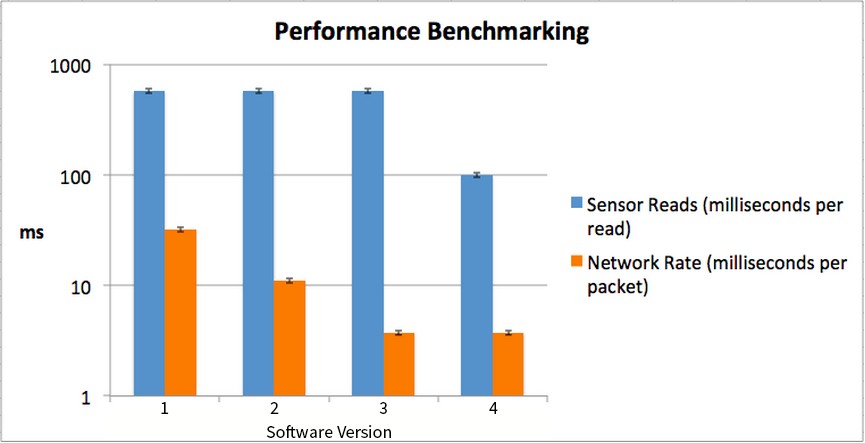
\includegraphics[width=3in]{images/graph.png}
  \end{center}
  \caption{Network and sensor performance of various eKwip "models?"}
  \label{fig:graph}
\end{figure}






\begin{figure}[h]
  \begin{center}
    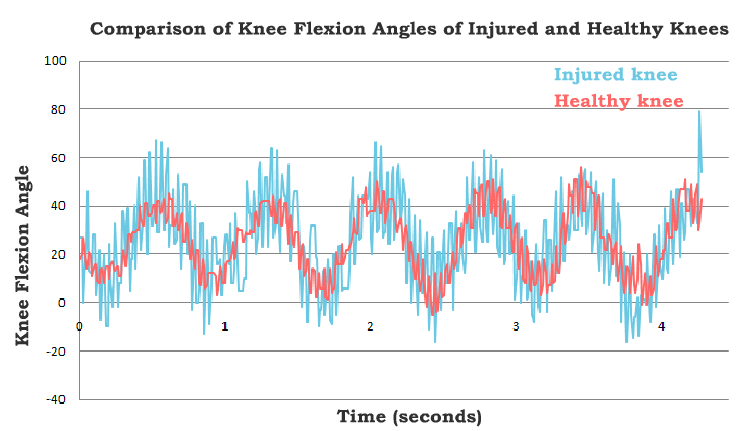
\includegraphics[width=3.4in]{images/results_graph.PNG}
  \end{center}
  \caption{Block diagram of eKwip system}
  \label{fig:results_graph}
\end{figure}